\subsubsection{Stromform}
Folgende Einstellungen wurden bei diesem Versuch vorgenommen:
\begin{itemize}
\item Winkel $\alpha = 0°$
\item Wechselrichter ist mit dem Netz synchronisiert.
\end{itemize}

Die Spannung $U_L$ ist die zeitliche Ableitung des Stromes multipliziert mit der Induktivität.
\begin{center}
$U_L = L * \frac{di}{dt}$
\end{center}

\begin{figure}[H]
  \begin{center}
  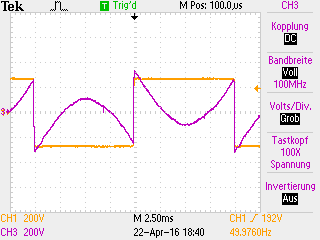
\includegraphics[width=0.48\textwidth]
  {pic/6_1_grundfrequenztaktung/6_1_1_stromform/ALL0001/F0001TEK.png}
  \caption{$U_A$ (orange) , $U_L$ (violett)}
  \label{fig:6_1_1_1}
  \end{center}
\end{figure}


Die Strom $I_L$ ist das Integral der Spannung $U_L$ geteilt durch die Induktivität, zuzüglich des Startwerts.
\begin{center}
$I_L = \frac{1}{L} * \int U_L dt$
\end{center}
\begin{figure}[H]
  \begin{center}
  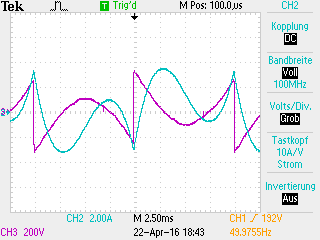
\includegraphics[width=0.48\textwidth]
  {pic/6_1_grundfrequenztaktung/6_1_1_stromform/ALL0002/F0002TEK.png}
  \caption{$U_L$ (violett), $I_{L1}$ (blau)}
  \label{fig:6_1_1_2}
  \end{center}
\end{figure}

Nur die Wechselrichterspannung $U_A$ enthält harmonische Oberschwingungen, nämlich alle ungeraden. Anhand der Tabelle \ref{tab:harm_wr} sieht man, dass die Amplitude der v-ten Oberschwingung jeweils um $1/v$ kleiner ist als die der Grundschwingung.

\begin{table}[h]
  \centering
  \begin{tabular}{ l | l | l }
    \hline 
    Harmonische  & Wert & Einheit \\
    \hline \hline
    $U_A$ eff. & 253  &  V\\
    \hline
    $U_A$ 01   & 220  &  V\\  
    \hline 
    $U_A$ 02   & 0.1  &  \%\\  
    \hline
    $U_A$ 03   & 33.5 &  \%\\  
    \hline
    $U_A$ 05   & 20   &  \%\\  
    \hline
    $U_A$ 07   & 14   &  \%\\  
    \hline
    $U_A$ 09   & 11   &  \%\\  
    \hline
  \end{tabular}
  \caption{Harmonische der Wechselrichterspannung $U_A$}
  \label{tab:harm_wr}
\end{table}

\begin{table}[h]
  \centering
  \begin{tabular}{ l | l | l }
    \hline 
    Harmonische  & Wert & Einheit \\
    \hline \hline
    $U_A$ 01   & 220  &  V\\  
    \hline 
    $U_A$ 03   & 0.1  &  \%\\  
    \hline
  \end{tabular}
  \caption{Harmonische der Netzspannung}
  \label{tab:harm_netz}
\end{table}



\clearpage